% !TEX program = xelatex
% Copyright 2026 Chen Jiaqi (GitHub: @H15teve)
% Distributed under LPPL 1.3c or later; maintenance status: maintained.
% Current Maintainer: Chen Jiaqi (GitHub: @H15teve).
% This work consists of the files listed in LPPL-MANIFEST.txt.
%==================================================================
%  paper-example-overleaf.tex — Overleaf 免费版（10 秒）编译入口
%  与 paper-example.tex 内容相同，但参考文献改用标准 thebibliography
%  环境，不加载 biblatex，避免 preamble 阶段加载 gb7714 样式链超时。
%  真实写作请使用 paper-example.tex（biblatex + biber）。
%==================================================================
\documentclass[UTF8,twoside,a4paper,fontset=none]{ctexart}
% overleaf: 锁定 TeX Live 自带字体并跳过非必要宏包，适合 Overleaf 免费版 10 s 限制。
\usepackage[fontset=overleaf,fastcompile]{csee}
\graphicspath{{figures/}}

\cseeheader{中国电机工程学报}{Proceedings of the CSEE}

\begin{document}

%================ 篇首通栏题头 =================
\begin{cseefrontmatter}
\cseearticlemeta
  {10.13334/j.0258-8013.pcsee.XXXXXX}
  {0258-8013 (2026) XX-XXXX-XX}
  {TM\,721}
\cseetitle{中文标题}
\cseeauthor{作者姓名}
\cseeaffiliation{（1．作者单位，地址　邮编）}
\cseetitleEN{English Title}
\cseeauthorEN{AUTHOR Name}
\cseeaffiliationEN{(Author Affiliation)}
\end{cseefrontmatter}

% 在首页左栏开始处登记基金块；模板按实际内容高度预留栏底空间。
\cseefund
  {基金项目名称（项目编号示例：XXXXXXXX\cseefundbreak XX）}
  {Fund project name (Grant No. XXXXXXXX\cseefundbreak XX).}

%================ 双栏正文(ABSTRACT 是闭合后第一段) =================
\begin{cseeabstractEN}
English abstract content here.
\end{cseeabstractEN}
\cseekeywordsEN{keyword1; keyword2; keyword3}

\begin{cseeabstract}
中文摘要内容。
\end{cseeabstract}
\cseekeywords{关键词1；关键词2；关键词3}

\section{引言}
直流输电技术在电力系统中的应用日益广泛\cite{ref1,ref7}。本文研究相关内容。

\subsection{研究背景}
已有研究\cite{ref2,ref4}表明相关方向的重要性。

\subsubsection{三级标题}
正文内容。

\section{方法}
正文内容。

\begin{equation}
\label{eq:1}
x = \sum_{i=1}^{n} a_i
\end{equation}

\begin{table}[!ht]
  \centering
  \cseetablecaption{表题}{Table caption}\label{tab:1}
  \cseetabletext
  \begin{tabular}{cc}
    \toprule
    列1 & 列2 \\
    \midrule
    数据1 & 数据2 \\
    \bottomrule
  \end{tabular}
\end{table}

\begin{figure}[!ht]
  \centering
  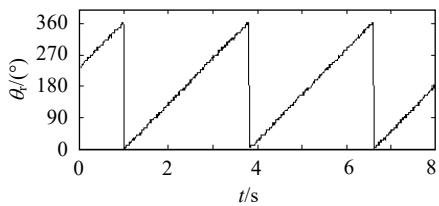
\includegraphics[width=0.9\linewidth]{figA1.jpg}
  \cseefigurecaption{图题}{Figure caption}\label{fig:1}
\end{figure}

% 在文末结构前排出尚未落版的图表，避免图表越过参考文献。
\clearpage
\cseeacknowledgment{致谢内容。}

%================ 参考文献（手写 thebibliography，不依赖 biber）=================
\renewcommand{\refname}{参考文献}
\begin{thebibliography}{99}
\bibitem{ref1} 葛俊，童陆园，耿俊成，等．TCSC暂态过程中晶闸管导通角特性的研究[J]．电网技术，2001，25(7)：18-22．
\bibitem{ref2} 张贤达．现代信号处理[M]．北京：清华大学出版社，2002：179-193．
\bibitem{ref4} Anderson P M，Agrawal B L，Van Ness J E．Subsynchronous Resonance in Power Systems[M]．New York：IEEE Press，1990：35-68．
\bibitem{ref7} Sharma C．Modeling of an island grid[J]．IEEE Transactions on Power Systems，1998，13(3)：971-978．
\end{thebibliography}

%================ 附录 =================
\cseeappendixhead[A]
附录内容。

\cseebiography[\#\#\#]{author_photo.jpg}{作者姓名（19XX），性别，学位，职称，主要研究方向；author@example.com。}

\end{document}
